En la Figura \ref{doc_contents} se puede apreciar la tabla de contenidos de la documentación generada para el paquete.
En el siguiente enlace https://corvus96.github.io/PyTwoVision/html/index.html se puede encontrar la documentación completa del mismo.
\begin{figure}[H]
    \centering
    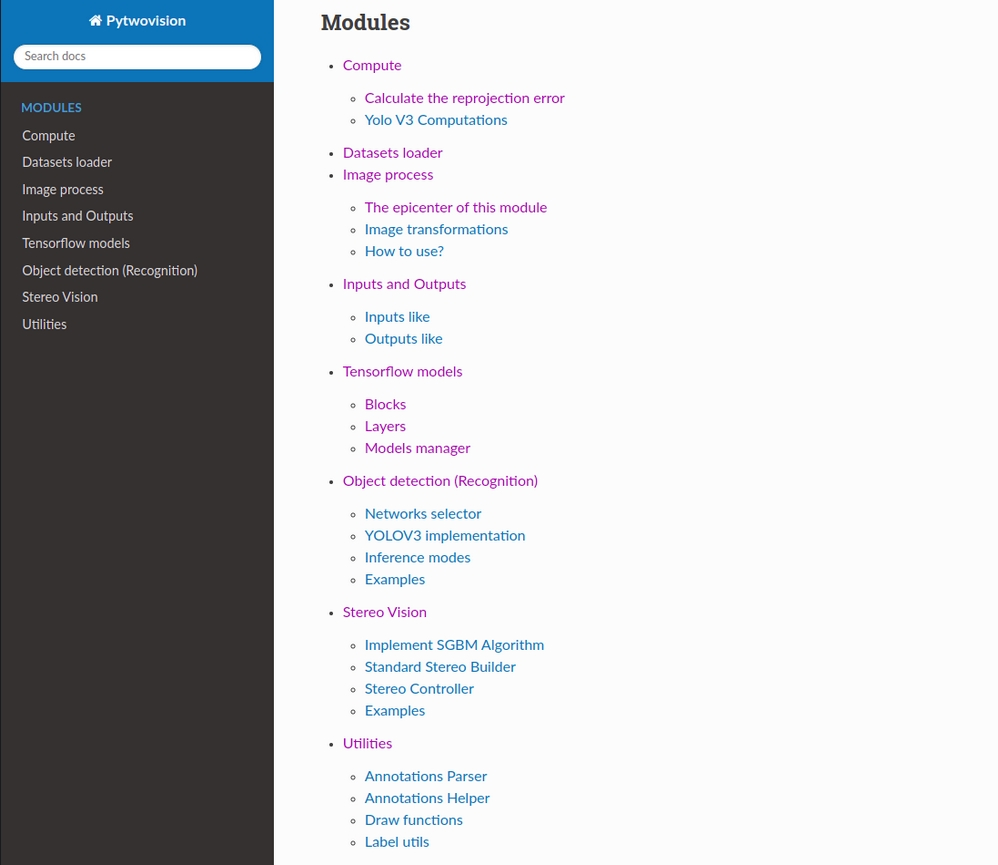
\includegraphics[scale=0.5]{Recursos/doc_contents.jpg}
    \caption{Tabla de contenidos de la documentación del paquete}
    \label{doc_contents}
\end{figure}
En el enlace https://github.com/corvus96/PyTwoVision/tree/master/tutorials se encuentran los tutoriales desarrollados, los cuales pueden ser ejecutados en Jupyter notebooks o en Google Colab. 
\begin{figure}[H]
    \centering
    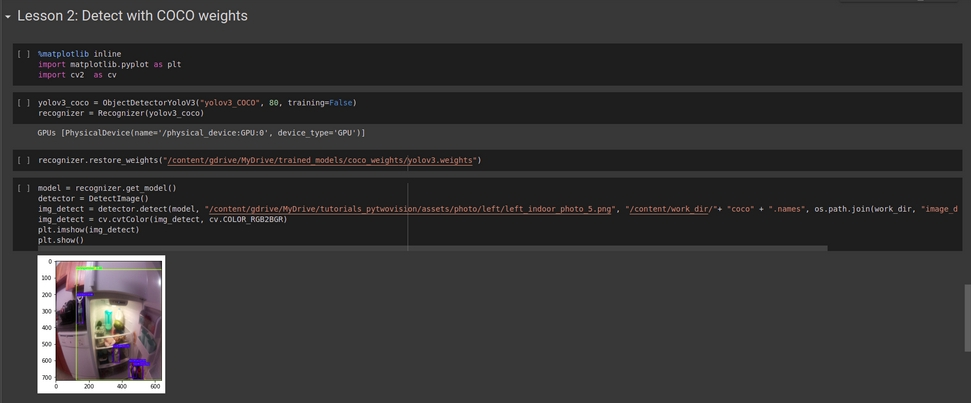
\includegraphics[scale=0.6]{Recursos/lesson_example.jpg}
    \caption{Extracto del tutorial de implementación de YOLO}
    \label{fig:my_label}
\end{figure}